\taskpic{Вагон длиной $4L$ и шириной $L$, стоящий на абсолютно гладких
  рельсах, заполнен водой до высоты $L$. В нем со дна всплывает легкий
  куб с ребром $L$. На какое расстояние и в какую сторону от точки А
  сдвинется вагон после успокоения воды, если плотность вещества куба
  в два раза меньше плотности воды, а масса пустого вагона равна массе
  налитой в него воды?}
{
  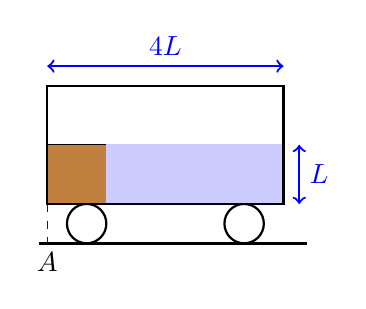
\begin{tikzpicture}
    \draw[very thick] (0.4,0.5) -- ++(3.4,0);
    \draw[thick] (1,0.75) circle (0.25);
    \draw[thick] (3,0.75) circle (0.25);
    \draw[fill=brown] (0.5,1) rectangle +(1.5/2,1.5/2);
    \draw[fill=blue!20,draw=blue!20] (0.5+1.5/2,1) rectangle +(4.5/2,1.5/2);
    \draw[<->,blue,thick] (0.5,2.75) -- ++(3,0) node [midway,above]
    {$4L$};
    \draw[<->,blue,thick] (3.7,1) -- ++(0,1.5/2) node[midway,right] {$L$};
    \draw[blue,dashed] (0.5,1) -- ++(0,-0.5) node [black,below] {$A$};
    \draw[thick] (0.5,1) rectangle ++(3,1.5);
  \end{tikzpicture}
}
